%
% 公立はこだて未来大学卒業研究中間報告書[全コース対応版]
%
%         ファイル名："sample.tex"
%
% !TEX encoding = UTF-8
% !TEX program = lualatex
\documentclass[11pt]{ltjarticle}
\usepackage{funinfosys}
\usepackage{url}
\usepackage{graphicx}
\author{%
1022179 西野理希\\指導教員 : イアン・フランク
}
%\course{Information Systems Course}
%\course{Advanced ICT Course} %% 高度ICTコースの場合はこちらを使用
%\course{Information Design Course} %% 情報デザインコースの場合はこちらを使用
\course{Complex Systems Course} %% 複雑系科学コースの場合はこちらを使用
%\course{Intelligent Systems Course} %% 知能システムコースの場合はこちらを使用
\title{作るか、選ぶか?\\教員による提示方法が教育動画の価値認識に与える影響}
\etitle{Create or Curate?\\ How Instructor Framing Shapes the Value of Educational Video}
\eauthor{NISHINO Riki}
\abstract{大学教育では教育動画の活用が広がっている一方，教員による独自の動画制作には時間や技術的な負担が伴う．本研究では，動画の制作や選定そのものの教育効果ではなく，教員による動画の提示方法が学習者の価値認識に与える影響を検討する．大学生を対象とするオンライン実験を計画し，参加者を制作条件，選定条件，中立条件の3条件に無作為に割り当てる．各条件では同じ教育動画3本を使用し，動画の由来に関する説明のみを変更する．各動画の視聴後に7段階のアンケートと理解度テストを実施し，教材としての適切性，授業への採用価値，他の学生への推奨評価から構成する主観的な教育的価値を主要指標として比較する．また，終了後には提示された説明の記憶と信憑性を確認する．現在は生成AIの文章生成を題材とした動画の脚本初稿を作成しており，今後は動画1本を用いた実験手順と質問紙の試行を検討する．}
\keywords{教育動画，キュレーション，提示方法，価値認識}
\eabstract{Educational videos are increasingly used in higher education, while producing original materials can place demands on instructors. This study examines how instructor framing affects students’ perceived value of educational videos, rather than the educational effectiveness of curation itself. In a planned online experiment, university students will be randomly assigned to one of three framing conditions: instructor-created, instructor-selected, or neutral. All conditions will use the same three videos. After each video, participants will complete seven-point ratings and a comprehension test. The primary outcome is perceived educational value, assessed through suitability as course material, value for classroom use, and willingness to recommend the video. Participants will also report what they remember being told about the videos’ origin and whether they believed it. A draft script about generative AI has been prepared.}
\ekeywords{Educational Videos, Curation, Framing, Perceived Value}
\begin{document}
\maketitle
%\vspace*{-.5cm}

\section{背景と目的}

近年，大学教育においてオンライン学習環境の普及に伴い，教育動画の活用が広がっている．Noetelら\cite{noetel2021}は，高等教育における教育動画が学習成果の向上に寄与することを報告している．一方，教育動画の制作には時間や技術が必要であり，教員が独自に制作することには負担が伴う．そのため，既存の動画を教育目的に応じて選定・活用するキュレーションも，教材を準備する方法の一つとなる．

教育動画の活用において，教員が自ら教材を制作することと，既存の教材を選定することは，異なる形の教育的な関与である．しかし，こうした教員の関与に関する情報が，学習者による教材の評価にどのような影響を与えるかについては，十分に明らかになっていない．

本研究では，教員による教育動画の提示方法が，学習者の価値認識に与える影響を検討することを目的とする．具体的には，同一の教育動画を「教員が制作した動画」「教員が選定した動画」「由来を説明しない動画」として提示する3条件を設定し，学習者が感じる教育的価値，有用性，信頼性などの評価を比較する．これにより，動画の内容を統一したうえで，教員の関与に関する説明の違いが学習者の評価に与える影響を明らかにすることを目指す．

\section{複雑系コースにおける本研究の位置づけ}
複雑系コースでは，自然や社会に見られる現象の法則性を分析し，実世界の課題に適用する能力の育成を目指している．本研究では，教育動画に対する教員の関与の提示方法と，学習者の価値認識との関係を比較実験によって検討する．提示条件を操作して得られた評価データを定量的に分析することで，教員の関与に関する情報が学習者の評価に及ぼす影響を調べ，教育現場における教材の提示方法について知見を得ることを目指す．


\section{関連研究}

教育動画の有効性について，Noetelら\cite{noetel2021}は，高等教育における教育動画の活用が学習成果の向上に寄与することを報告している．一方，Liesa-Orúsら\cite{liesa2023}は，大学教員のデジタル能力に関する課題を報告している．教育動画の制作においても，こうしたデジタル能力が求められるため，既存の教材を活用する方法について検討する意義がある．

既存の教材を活用する方法として，DeschaineとSharma\cite{deschaine2015}は，デジタルキュレーションを教育目的に応じた学習資源の選定・整理・共有の活動として位置づけている．また，Flintoffら\cite{flintoff2014}は，教育や研究におけるデジタルキュレーションの重要性を論じている．これらの研究は，教材の制作だけでなく，既存の教材を選定することも教員の役割の一つであることを示している．

一方，HovlandとWeiss\cite{hovland1951}は，情報源の信頼性が情報の受容に影響することを示している．また，RamlatchanとWatson\cite{ramlatchan2020}は，オンライン講義動画の提示方法が，学習者による教員の信頼性や心理的近接性の評価に影響することを報告している．これらの研究は，情報の内容だけでなく，その提示方法や情報源に対する認識も受け手の評価に関係することを示している．

本研究では，これらの知見を踏まえ，同一の教育動画に対して「教員が制作した」「教員が選定した」という異なる説明を与え，学習者による評価を比較する．これにより，教材の実際の制作・選定方法ではなく，教員の関与に関する説明が教育動画の価値認識に与える影響を検討する．



\section{研究方法}

\subsection{実験計画}

本研究では，大学生を対象としたオンライン実験を計画している．参加者を制作条件，選定条件，中立条件の3条件に無作為に割り当て，教員による動画の提示方法の違いを比較する．各条件で使用する説明文は以下のとおりである．

\begin{itemize}
  \item 制作条件（Create）：「これは，この授業で使用するために担当教員が制作した動画です．」
  \item 選定条件（Curate）：「これは，この授業で使用するために担当教員が選定した動画です．」
  \item 中立条件（Neutral）：「これは，この授業で使用する動画です．」
\end{itemize}

各参加者は，割り当てられた条件のもとで，AIリテラシーに関する約3分間の教育動画を3本視聴する．動画は全条件で共通とし，提示順序は可能な範囲で均衡させる．条件間では動画そのものを変更せず，教員の関与に関する説明のみを操作する．

\subsection{評価指標}

各動画の視聴後，7段階評価によるアンケートと内容理解度テストを実施する．本研究では，学習者が主観的に評価する授業教材としての教育的価値を主要評価指標とする．教材としての適切性，授業への採用価値，他の学生への推奨評価の3項目を測定し，その平均得点を用いることを検討している．

副次評価指標として，学習上の有用性，説明内容の信頼性，満足度，学習意欲を各1項目で測定する．また，各動画に2〜3問の選択式理解度テストを設け，内容理解の状況を補助的に確認する．

全動画の評価終了後には，動画の由来についてどのように説明されたと記憶しているか，また，その説明をどの程度信じていたかを確認する．これにより，提示した説明が参加者にどのように受け止められたかを把握する．

\begin{figure*}[t]
  \centering
  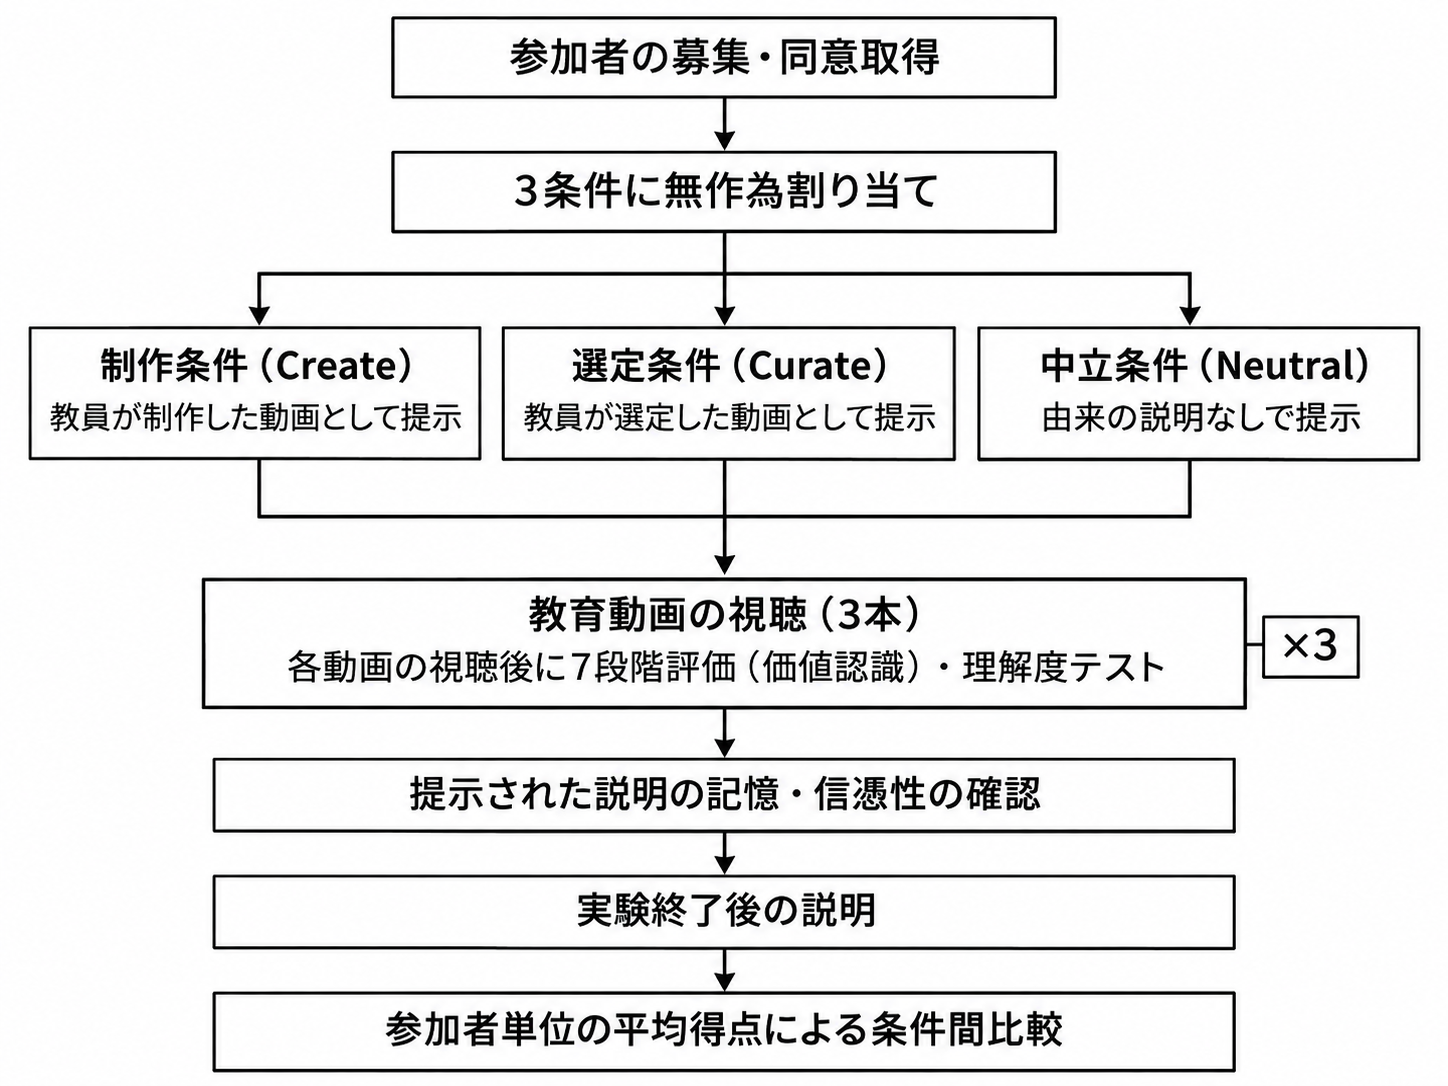
\includegraphics[
    width=0.85\textwidth,
    height=0.35\textheight,
    keepaspectratio]{images/fig_1.png}
  \caption{実験フロー（生成AIを用いて作成）}
  \label{fig:experiment_flow}
\end{figure*}


\subsection{分析方法}

主要な分析では，各参加者が3本の動画に対して付けた教育的価値の評価得点を平均し，参加者単位の得点を算出する．これを用いて制作条件と選定条件の評価の差を比較し，中立条件との比較は副次的に検討する．

また，動画ごとの評価の違いや参加者数などを踏まえ，必要に応じて線形混合効果モデルによる追加分析を検討する\cite{baayen2008}．結果は条件間の評価得点の差とその不確実性を考慮して解釈する．

\subsection{研究上の制約と倫理的配慮}

本研究では，参加者数や使用する動画の種類が限られる可能性があるため，得られた結果の一般化には制約がある．また，独自に設定した評価項目の妥当性や，動画間の品質・難易度の違いについても考慮する必要がある．

さらに，提示条件によっては，動画の実際の制作経緯とは異なる説明を参加者に与える可能性がある．そのため，参加者への説明や同意取得，実験終了後の説明など，研究倫理上の配慮について検討する．



\section{現在の進捗と今後の計画}

\subsection{刺激動画の制作状況}

現在，実験に使用する教育動画の準備を進めている．動画の題材には生成AIを検討しており，「生成AIはどのように回答を作るのか？」をテーマとした動画の脚本初稿を作成した．

本動画は，AI初学者の大学生を対象に，生成AIによる文章生成の基本的な仕組みを説明するものである．図解・アニメーションとナレーションを用いた約3分間の構成を想定し，全5シーン・19カットに分けて映像内容や演出を設計した．特に，文章を処理する単位であるトークンと，次のトークンの予測・追加を繰り返す文章生成の仕組みを中心に扱っている．

\subsection{今後の計画}

今後は，まず1本の教育動画を完成させ，質問紙と実験手順を組み合わせた試行を検討する．この試行では，提示条件の説明，動画視聴，理解度テスト，アンケート回答までの一連の手順を確認し，本実験に向けた課題を把握することを目指す．

その後，残りの教育動画の準備を進めるとともに，参加者の募集方法や実験手順を具体化する．本実験では，収集した評価データを提示条件間で比較し，教員による説明の違いが学習者の価値認識に与える影響を分析する．



\section{結言}

本研究では，教員による教育動画の提示方法が学習者の価値認識に与える影響を検討する．現在は，制作・選定・中立の3条件による比較実験の設計を進め，評価指標や分析方法の検討と，実験に使用する教育動画の脚本作成を行っている．今後は，動画1本を用いた試行によって実験手順や質問項目を確認し，残りの動画の準備とオンライン実験の実施に向けた作業を進める．これにより，教員の関与に関する説明の違いが学習者による教育動画の評価に与える影響を明らかにすることを目指す．



\begin{thebibliography}{99}

\bibitem{noetel2021}
Noetel, M., et al. (2021).
Video improves learning in higher education:
A systematic review.
\textit{Review of Educational Research},
91(2), 204--236.
\url{https://doi.org/10.3102/0034654321990713}

\bibitem{liesa2023}
Liesa-Orús, M., Lozano Blasco, R.,
\& Arce-Romeral, L. (2023).
Digital competence in university lecturers:
A meta-analysis of teaching challenges.
\textit{Education Sciences}, 13(5), 508.
\url{https://doi.org/10.3390/educsci13050508}

\bibitem{deschaine2015}
Deschaine, M. E., \& Sharma, S. A. (2015).
The five Cs of digital curation:
Supporting twenty-first-century teaching
and learning.
\textit{InSight: A Journal of Scholarly Teaching},
10, 19--24.
\url{https://doi.org/10.46504/10201501de}

\bibitem{flintoff2014}
Flintoff, K., Mellow, P.,
\& Clark, K. P. (2014).
Digital curation: Opportunities for learning,
teaching, research and professional development.
In \textit{Proceedings of the 23rd Annual
Teaching Learning Forum}.
University of Western Australia.

\bibitem{hovland1951}
Hovland, C. I., \& Weiss, W. (1951).
The influence of source credibility on
communication effectiveness.
\textit{Public Opinion Quarterly},
15(4), 635--650.
\url{https://doi.org/10.1086/266350}

\bibitem{ramlatchan2020}
Ramlatchan, M., \& Watson, G. S. (2020).
Enhancing instructor credibility and
immediacy in online multimedia designs.
\textit{Educational Technology Research
and Development}, 68(1), 511--528.
\url{https://doi.org/10.1007/s11423-019-09714-y}

\bibitem{baayen2008}
Baayen, R. H., Davidson, D. J.,
\& Bates, D. M. (2008).
Mixed-effects modeling with crossed
random effects for subjects and items.
\textit{Journal of Memory and Language},
59(4), 390--412.
\url{https://doi.org/10.1016/j.jml.2007.12.005}

\end{thebibliography}
\end{document}
%
%
% EOF
